\subsection{Sự hội tụ của chuỗi Markov dưới góc nhìn ma trận}
%%--------frame 1-------
\begin{frame}{Sự hội tụ của chuỗi Markov dưới góc nhìn ma trận}
    \begin{mydef*}{}
        Một chuỗi Markov được gọi là \textbf{chuỗi chính tắc} nếu tồn tại một số $n \geq 1$ sao cho các phần tử của $\mathbf{P}^n$ đều dương (lớn hơn 0).
    \end{mydef*}
    \begin{itemize}
        \item[\bullet] Xét chuỗi Markov sau:
\begin{figure}[H]
\centering
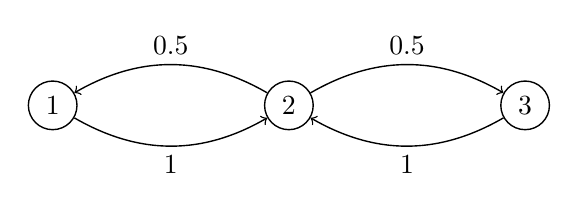
\begin{tikzpicture}[-> , line width=0.5 pt ,node distance =2 cm]
    % \tikzstyle{every node}=[font=\large]
    
    \node[circle, draw] (1) at (0,0) {1};
    \node[circle, draw] (2) at (3,0) {2};
    \node[circle, draw] (3) at (6,0) {3};

    \path (1) edge [bend right] node [below] {$1$} (2);
    \path (2) edge [bend right] node [above] {$0.5$} (1);
    \path (2) edge [bend left] node [above] {$0.5$} (3);
    \path (3) edge [bend left] node [below] {$1$} (2);
    
\end{tikzpicture}
\caption{Ví dụ chuỗi Markov} 
\label{fig:grapheg}
\end{figure}

\item[\bullet] Dựa vào đồ thị ta có ma trận chuyển tiếp:
$$
\mathbf{P} = \begin{bmatrix}
    0 & 1 & 0 \\
    0.5 & 0 & 0.5 \\
    0 & 1 & 0
\end{bmatrix}
$$
    \end{itemize}
\end{frame}

%%--------frame 2-------
\begin{frame}{Sự hội tụ của chuỗi Markov dưới góc nhìn ma trận}
\vfill
    \begin{mytheo*}{}
        Nếu chuỗi markov là một chuỗi chính tắc và ma trận chuyển tiếp $\mathbf{P}$ chéo hoá được thì tồn tại phân phối bất động $\pi$. Đặt $e$ là vector riêng ứng với trị riêng bằng 1 của ma trận $\mathbf{P}^T$, khi đó $\pi = e^T$.
    \end{mytheo*}
    \vfill
\end{frame}
%%--------frame 3-------
\begin{frame}{Sự hội tụ của chuỗi Markov dưới góc nhìn ma trận}
    \begin{myproof*}{}
        Vì chúng ta vẫn thường thao tác với không gian cột, nên bài chứng minh sẽ xét với ma trận chuyển vị từ hàng thành cột để dễ dàng hình dung hơn.
    \begin{itemize}
        \item[\bullet] Xét ma trận Markov $\mathbf{P}$ chéo hoá được thành $\mathbf{P} = U D U^{-1}$, ta có $\mathbf{P}^T$ cũng chéo hoá được, chứng minh như sau: 
        \begin{align}
            \mathbf{P}^T = (U D U^{-1})^T = (U^{-1})^T D^T U^T = (U^{T})^{-1} D^T U^T
        \end{align}

        \item[\bullet] Đặt $(U^{-1})^T = X$, đồng thời lại có $D^T = D$, từ đó ta được:
        \begin{align}
            \mathbf{P}^T = (U^{-1})^T D^T U^T = X D X^{-1}
        \end{align}

        \item[\bullet] Suy ra $\mathbf{P}^T$ chéo hoá được. Xét ma trận $\mathbf{P}^T$, $X$ là ma trận có các cột là các vector riêng, cột đầu tiên là vector riêng ứng với $\lambda_1 = 1$ , ta được:
        \begin{align}
            \mathbf{P}^T = X D X^{-1}
        \end{align}
        \end{itemize}
    \end{myproof*}
\end{frame}

%%--------frame 4-------
\begin{frame}{Sự hội tụ của chuỗi Markov dưới góc nhìn ma trận}

\begin{myproof*}{(tt)}
    \begin{itemize}
         \item[\bullet] Với $\textbf{x}_i$ là các cột của $X, \lambda_i$ là các trị riêng tương ứng với $\textbf{x}_i$, ta được
            \begin{align}
                X = \begin{bmatrix}
                \textbf{x}_1& \textbf{x}_2 & \dots& \textbf{x}_n
                \end{bmatrix}, D = \begin{bmatrix}
                \lambda_1&0& \dotsb &0\\
                0&\lambda_2& \dotsb &0\\
                \vdots & \vdots & \ddots & \vdots\\
                0&0&\dotsb & \lambda_n
                \end{bmatrix}
            \end{align}
        \item[\bullet] Lúc này, $\textbf{x}_i$ là các cột của $X$, phân phối ban đầu $\pi_0$ sẽ được biểu diễn thành tổ hợp tuyến tính của $x_i$ như sau (vì $P^T$ chéo hoá được nên ta sẽ có các vector $x_i$ là cớ sở của không gian $R^{n\text{x}n}$):
        \begin{align}
            \pi_0^T &= c_1 \textbf{x}_1 + c_2 \textbf{x}_2 + ... + c_n \textbf{x}_n \\
            \pi_0^T &= 
            \begin{bmatrix}
                \textbf{x}_1 & ... & \textbf{x}_n 
            \end{bmatrix} 
            \begin{bmatrix}
                c_1 \\
                \vdots \\
                c_n
            \end{bmatrix}\\
            \textbf{c} &= X^{-1} \pi_0^T
        \end{align}
    \end{itemize}
\end{myproof*}
\end{frame}
%%--------frame 5-------
\begin{frame}{Sự hội tụ của chuỗi Markov dưới góc nhìn ma trận}
    \begin{myproof*}{(tt)}
    \begin{itemize}
        \item[\bullet] Vector trạng thái sau thời gian $k+1$:
        \begin{align}
            \pi_{k+1} &= \pi_0 \mathbf{P}^k \\
            \Leftrightarrow \hspace{10pt} \pi_{k+1}^T &= (\mathbf{P}^T)^k \pi_0^{T} \\
            \Leftrightarrow \hspace{10pt} \pi_{k+1}^T &= X D^k X^{-1} \pi_0^{T} \\
            \Leftrightarrow \hspace{10pt} \pi_{k+1}^T &= X D^k \textbf{c}
        \end{align}
    \item[\bullet] Ta có:
        \begin{align}
            X D^k =  \begin{bmatrix}
            \textbf{x}_1& \textbf{x}_2 & \dots& \textbf{x}_n
            \end{bmatrix} 
            \begin{bmatrix}
            \lambda_1^k&0& \dotsb &0\\
            0&\lambda_2^k& \dotsb &0\\
            \vdots & \vdots & \ddots & \vdots\\
            0&0&\dotsb & \lambda_n^k
            \end{bmatrix}
        \end{align}
    \end{itemize}
    \end{myproof*}
\end{frame}
%%--------frame 6-------
\begin{frame}{Sự hội tụ của chuỗi Markov dưới góc nhìn ma trận}
    \begin{myproof*}{(tt)}
    \begin{itemize}
        \item[\bullet] Sử dụng phương pháp nhân hai ma trận (ma trận này nhân với từng cột ma trận kia), ta được:
        \begin{align}
            X D^k =  
            \begin{bmatrix}
            \lambda_1^k\textbf{x}_1& \lambda_2^k\textbf{x}_2 & \dots&\lambda_n^k\textbf{x}_n
            \end{bmatrix} 
        \end{align}

        \item[\bullet] Cùng với quy ước $\lambda_1 = 1$, ta suy ra:
        \begin{align}
            \pi_{k+1}^T &= X D^k C = \begin{bmatrix}
            \lambda_1^k\textbf{x}_1& \lambda_2^k\textbf{x}_2 & \dots&\lambda_n^k\textbf{x}_n
            \end{bmatrix} \begin{bmatrix}
                c_1 \\
                \vdots \\
                c_n
            \end{bmatrix}\\
            &= c_1\textbf{x}_1 + c_2 \lambda_2^k \textbf{x}_2 + ... + c_n \lambda_n^k \textbf{x}_n
        \end{align}
    \end{itemize}
    \end{myproof*}
\end{frame}

\begin{frame}{Sự hội tụ của chuỗi Markov dưới góc nhìn ma trận}
    \begin{myproof*}{(tt)}
    \begin{itemize}
     
        \item[\bullet] Như đã chứng minh ở trên, các trị riêng khác $1$ và $-1$ đều có trị tuyệt đối nhỏ hơn 1, chính vì thế khi $k$ càng tăng đến số vô cùng lớn, thì $\pi_{k+1}^T$ sẽ càng tiến gần về $c_1\textbf{x}_1$. Và đây chính là lí do cho sự ``hội tụ'' của các phân phối.

        \item[\bullet] Vậy mới một ma trận Markov chéo hoá được, các phân phối sẽ hội tụ dần về phân phối bất động với phân phối bất động chính là vector riêng tương ứng với trị riêng bằng $1$.
    \end{itemize}
    \end{myproof*}
    
\end{frame}